\section{Erfaring}
En samlet liste af erfaringen de to kandidater har indenfor feltet hyttebombing indenfor Polyteknisk Forening:

\subsection{Studiestarten}
\begin{enumerate}
\item Vektor 2006 \cite{bib:url:Beret2007}
\item CSK 2007\cite{bib:url:Beret2007}
\item CSK 2008\cite{bib:url:Beret2008}
\item Vektor 2008\cite{bib:url:Beret2008}
\item CSK 2009\cite{bib:url:Beret2009}
\item Vektor 2009\cite{bib:url:Beret2009}
\end{enumerate}

\subsection{Madhold}
\begin{enumerate}
\item vOPtur 2008\cite{bib:url:Beret2008}
\item Rustur 2009\cite{bib:url:Beret2009}
\item hyttetur ELKO nystartende 2010\cite{bib:url:Beret2010}
\item S-husets hyttetur 2011\cite{bib:url:Beret2011}
\item OPtur 2011\cite{bib:url:Beret2011}
\item Rustur 2011\cite{bib:url:Beret2011}
\item hyttetur ELKO nystartende 2011\cite{bib:url:Beret2011}
\item S-husets hyttetur 2012
\end{enumerate}


\subsection{Arrangør af ture}

\begin{enumerate}
\item Rustur 2006\cite{bib:url:Beret2007}
\item HerreHyggeHyttetur ELKO 2007 \cite{bib:url:Beret2007}
\item OPtur 2007\cite{bib:url:Beret2007}
\item Rustur 2007\cite{bib:url:Beret2007}
\item HerreHyggeHyttetur ELKO 2008\cite{bib:url:Beret2008}
\item OPtur 2008\cite{bib:url:Beret2008}
\item Rustur 2008\cite{bib:url:Beret2008}
\item hyttetur ELKO nystartende 2008\cite{bib:url:Beret2008}
\item HerreHyggeHyttetur ELKO 2009\cite{bib:url:Beret2009}
\item OPtur 2009\cite{bib:url:Beret2009}
\item Rustur 2009\cite{bib:url:Beret2009}
\item hyttetur ELKO nystartende 2009\cite{bib:url:Beret2009}
\item HerreHyggeHyttetur ELKO 2011\cite{bib:url:Beret2011}
\item HerreHyggeHyttetur ELKO 2012
\end{enumerate}

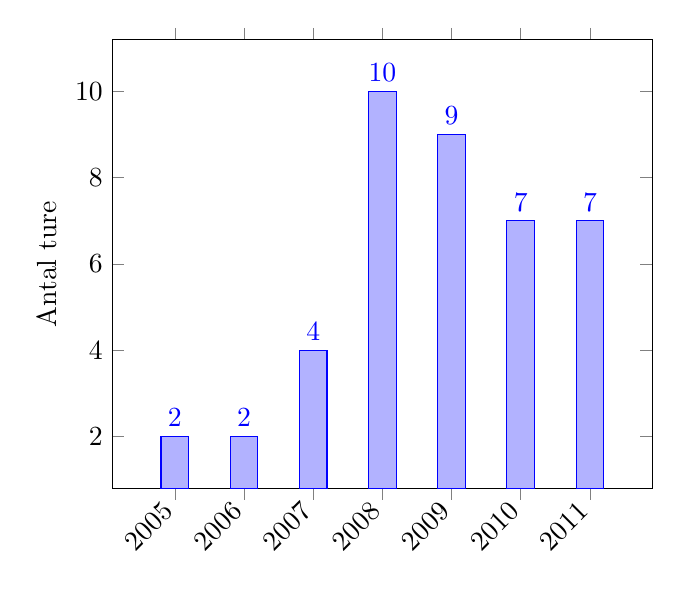
\begin{tikzpicture}
\begin{axis}[
ybar,
enlargelimits=0.15,
legend style={at={(0.5,-0.2)},
anchor=north,legend columns=-1},
ylabel={Antal ture},
symbolic x coords={2005, 2006, 2007, 2008, 2009, 2010, 2011, 2012},
xtick=data,
nodes near coords,
nodes near coords align={vertical},
x tick label style={rotate=45,anchor=east},
]
\addplot coordinates {(2005,2) (2006,2) (2007,4) (2008,10) (2009,9)(2010,7)(2011,7)};
\end{axis}
\end{tikzpicture}

\subsection{PF kompetancer}
\begin{enumerate}
\item Medlem ELKO 2006-2012\cite{bib:url:Beret2007},\cite{bib:url:Beret2008},\cite{bib:url:Beret2009},\cite{bib:url:Beret2010},\cite{bib:url:Beret2011}
\item Formand for ELKO rådet 2007-2009\cite{bib:url:Beret2007},\cite{bib:url:Beret2008},\cite{bib:url:Beret2009}
\item UddanelsesPolitisk Råd 2007-2012\cite{bib:url:Beret2007},\cite{bib:url:Beret2008},\cite{bib:url:Beret2009},\cite{bib:url:Beret2010},\cite{bib:url:Beret2011}
\item ISN Fotonik 2007-2012\cite{bib:url:Beret2007},\cite{bib:url:Beret2008},\cite{bib:url:Beret2009},\cite{bib:url:Beret2010},\cite{bib:url:Beret2011} , \cite{bib:url:ISNfoto}
\item Hegnet 2007->\cite{bib:url:Beret2007},\cite{bib:url:Beret2008},\cite{bib:url:Beret2009},\cite{bib:url:Beret2010},\cite{bib:url:Beret2011}
\item Hegnet Formand 2007-2008\cite{bib:url:Beret2007},\cite{bib:url:Beret2008}
\item Fællesrådet 2009+2011-2012\cite{bib:url:Beret2009},\cite{bib:url:Beret2010},\cite{bib:url:Beret2011}
\item Fællesrådets ForretningsUdvalg 2009-2012\cite{bib:url:Beret2009},\cite{bib:url:Beret2010},\cite{bib:url:Beret2011}
\item PF's Bestyrelse 2010\cite{bib:url:Beret2010}
\item Formand for ELKO rådet 2011-2012 \cite{bib:url:Beret2011}
\item Akademisk Råd (DTU) 2011-2012\cite{bib:url:Beret2011}
\end{enumerate}

\section{Hvad er Tha Bombs ikke}
\begin{enumerate}
\item Pædofil \cite{bib:url:Finn:Pedo}
\item Satan-tilbeder \cite{bib:url:Finn:Satan}
\item Dyrker sex med sovende kvinder \cite{bib:url:Finn:SovendeKvinder}
\item TV2 ansat \cite{bib:url:Finn:TV2}
\item Nazist\cite{bib:url:Finn:Nazist}
\end{enumerate}


Vi skal bruger DILD\cite{bib:url:Reklame:Dild}
\\
\\
Vi skal have en Anit Jehova Pæl \cite{bib:url:Reklame:Anti}
\\
\\
Tun i vand skal bruges \cite{bib:url:Reklame:Tun} rigeligt med tun i vand
\\
\\

%\begin{tikzpicture}
%\begin{axis}[view={60}{30}]
%\addplot3[mesh,z buffer=sort,
%samples=20,domain=-1:0,y domain=0:2*pi]
%({sqrt(1-x^2) * cos(deg(y))},
%{sqrt( 1-x^2 ) * sin(deg(y))},
%x);
%\end{axis}
%\end{tikzpicture}
%
%\begin{tikzpicture}
%\begin{axis}
%\addplot+[scatter,
%samples=500,scatter src=y]
%{x^-2};
%\end{axis}
%\end{tikzpicture}


